%!TEX root = ../../csuthesis_main.tex


\chapter{系统运行效果测试与分析}
\section{功能测试}
本系统采用现代化交互设计理念,其主界面布局如图4-1所示。


\begin{figure}[hbt]
	\centering
	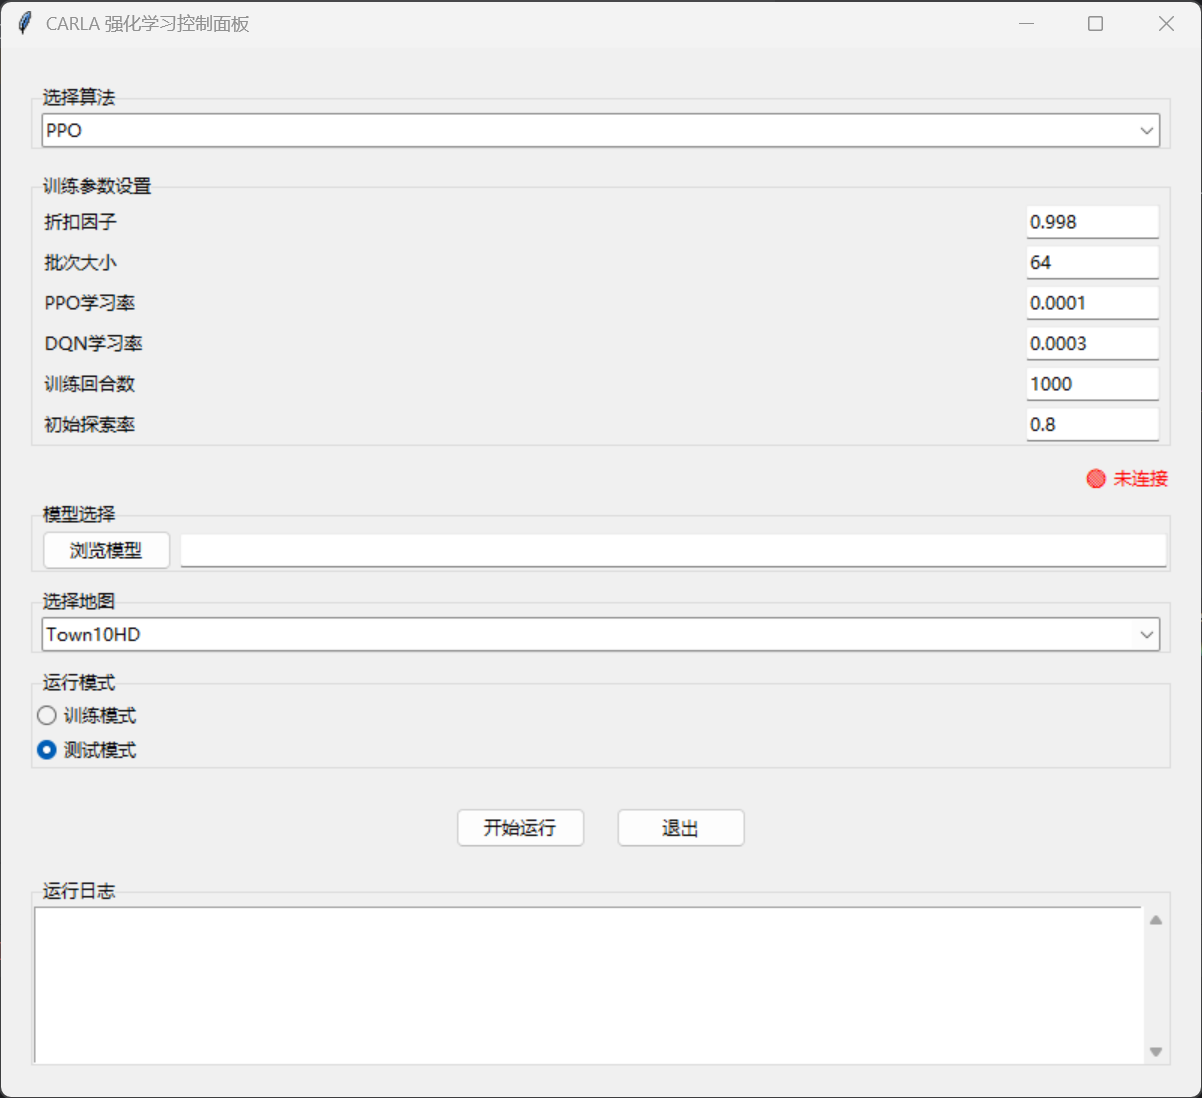
\includegraphics[width=0.8\linewidth]{用户界面.png}
	\caption{用户界面}
	\label{f.example}
\end{figure}

数字孪生的自动驾驶强化学习仿真系统图形用户界面即GUI,是基于Qt框架深度定制而成,它借助将多层级可视化组件和高响应交互逻辑进行无缝融合,构建起了一个全流程可视化闭环体系,该体系覆盖了仿真环境搭建、算法训练、策略验证以及结果分析等方面,界面采用功能分区式布局,上方功能区集成了核心控制模块与状态指示系统。用户可凭借下拉菜单以及交互式面板来选择强化学习算法,像PPO、SAC、DQN等,还可以加载预训练模型或者配置传感器参数,用户可以借助醒目的状态指示灯实时了解系统与Carla仿真引擎的通信状态,圆形指示灯以红绿双色编码直观反馈连接状态,当指示灯呈现红色时,意味着系统与Carla的TCP/IP通信链路没有成功建立或者出现了异常中断,这种情况可能是由端口冲突、仿真器未启动或者网络防火墙拦截所导致。而当切换为绿色常亮时,则代表双向通信通道已经稳定建立,底层数据交换线程正以毫秒级延迟同步车辆状态、环境信息以及控制指令。

下方运行日志区域采用了多级色彩编码的滚动文本框设计,可实时捕获系统运行过程中的关键事件流,并对其进行分类显示,其中INFO级日志会用白色字体记录常规操作,比如场景加载进度以及参数修改记录等,而WARNING级事件,像传感器数据丢包、奖励函数数值溢出等情况,会以黄色高亮的形式提示潜在风险。对于ERROR级故障,例如Carla连接超时、DRL策略崩溃等,则借助红色字体与震动警报相结合的方式来强化警示,该日志系统还内嵌了智能诊断引擎,当检测到“Carla Connection Failed”等高频错误时,会自动在日志末尾附加解决方案链,像检查1089端口占用情况、重启Carla服务进程等,并且支持点击错误代码直接跳转至对应配置页面。

在交互逻辑设计方面,系统借助事件驱动架构达成用户操作与仿真推演的紧密耦合,举例来说,当用户于功能区切换至“PPO算法训练”模式时,界面会自动激活相应的超参数编辑面板,右侧三维视窗会同步加载预设的训练场景,并且在日志区域生成“Training Mode Activated”的启动事件记录。在仿真推演进程中,用户可借助悬浮于3D视窗的透明控制条动态调节时间流速,而车辆轨迹、传感器数据流以及策略决策热以此来会以多图层叠加的形式实时进行渲染,形成“操作-响应-反馈”的强耦合交互循环,系统还引入了双向数据映射机制——点击日志中的特定事件可自动定位到对应时间戳的仿真场景回放,并且高亮显示碰撞瞬间的车辆姿态与障碍物位置,而三维视窗中的区域选择操作则会触发日志系统筛选相关时间区间的所有DRL动作分布与奖励函数构成的数据,以此实现跨模态信息的快速关联分析。这种设计提升了复杂算法调试的效率,凭借可视化闭环把抽象的强化学习过程转变为可直观干预的交互对象,降低了自动驾驶策略开发的技术门槛。

\begin{figure}[hbt]
	\centering
	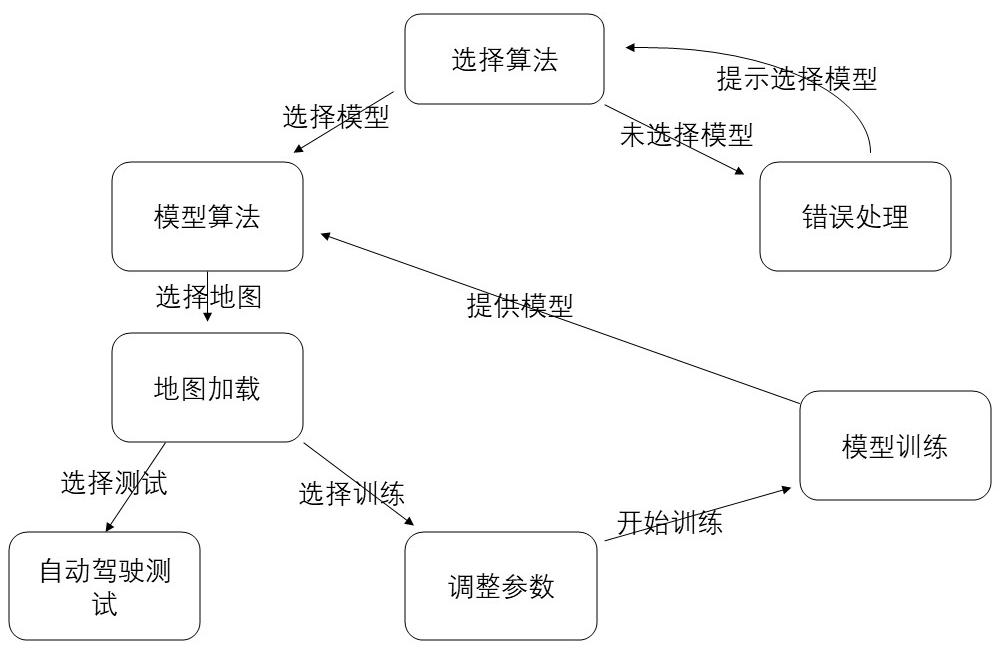
\includegraphics[width=0.8\linewidth]{交互逻辑演示.jpeg}
	\caption{交互逻辑演示图}
	\label{f.example}
\end{figure}

在数字孪生的自动驾驶强化学习仿真系统初始化状态时,用户可借助交互式控制面板逐步完成完整的训练或者测试流程配置,系统启动后默认处于“待命状态”,三维数字孪生视窗显示为空白场景,这时用户要先在算法选择模块里指定深度强化学习算法框架,比如PPO、SAC或者DQN,系统会自动加载相应算法的预设模型架构,像Actor - Critic网络拓扑、经验回放缓冲区配置等。要是用户没有进行模型选择,界面中央会动态弹出半透明警告层,依靠脉冲式高亮边框引导到算法选择区域,并且用语音合成技术播报“请选择强化学习算法以初始化策略网络”的提示消息,完成算法选择后,用户需在地图配置模块中从Carla支持的开放场景库,也就是Town01至Town07,或者自定义高精地图中选定训练或测试环境,系统会实时加载道路拓扑数据并在三维视窗中生成包含动态交通流、可变天气系统的数字孪生场景。

在选择“测试模式”时,用户要从模型仓库里挑选预训练权重文件,之后系统会自动把选定的模型部署到仿真环境中,并且在状态栏展示模型哈希值以及训练元数据,启动测试后,车辆会依据选定的策略在目标地图里自主行驶,界面右侧会同步展开多维度的监控面板:策略决策流会以热以此来的形式映射在鸟瞰视图上,动作选择概率分布会借助环形雷达图实时更新,安全评估模块会持续输出车道保持率、紧急制动频次等关键指标。要是切换到“训练模式”,用户可深度定制训练参数体系——借助滑动条精确调整学习率、折扣因子γ、探索率衰减曲线,也可以勾选高级选项来启用课程学习策略,设置渐进式的场景难度,参数确认完毕后,点击运行按钮会触发分布式训练管道,系统会自动分配计算资源并且在后台建立与 Carla 仿真的多线程通信链路,训练过程中用户可依靠悬浮式控制台动态调整参数权重,修改后的结果会实时注入训练进程而不会中断推演。

当模型训练完成后便会自动归档到模型仓库之中,用户可借助模糊搜索功能迅速定位到目标模型,系统会为每一个模型生成可视化的档案卡片,卡片上会展示训练损失曲线、场景借助率热以此来以及关键行为片段,所有用户自定义的模型都支持一键对比测试,系统会在相同场景下并行加载多个策略的推演过程,凭借画中画模式同步呈现不同模型的轨迹偏差、奖励累积差异等关键数据,为算法优化提供直观的基准参照。这样一种从配置到产出的一站式工作流设计,让那些即便没有编程经验的用户也可快速完成自动驾驶策略的迭代优化,而开发者则可以依靠开放API接口接入自定义算法模块,达成研究闭环的灵活扩展。
\subsection{算法选择功能}
本系统的一个核心功能模块是为用户打造开放式的强化学习算法交互框架,在图4-3所示的设计界面里,用户可借助可视化面板随意调用或者扩展算法库,系统预先集成了PPO、DQN等主流强化学习算法,每一种算法都配有图形化参数配置器,用户可以动态调整折扣因子γ、探索率ε等超参数,还可以经由CUDA加速的实时训练监控仪表盘观察Q值收敛状况。系统还开放了Python/C++双语言接口,支持用户以继承基类的形式植入自定义算法,系统会自动开展算法兼容性验证以及容器化封装,在模型训练阶段,用户可选定特定算法对自动驾驶感知 - 决策 - 控制全栈模型进行端到端训练。

\begin{figure}[hbt]
	\centering
	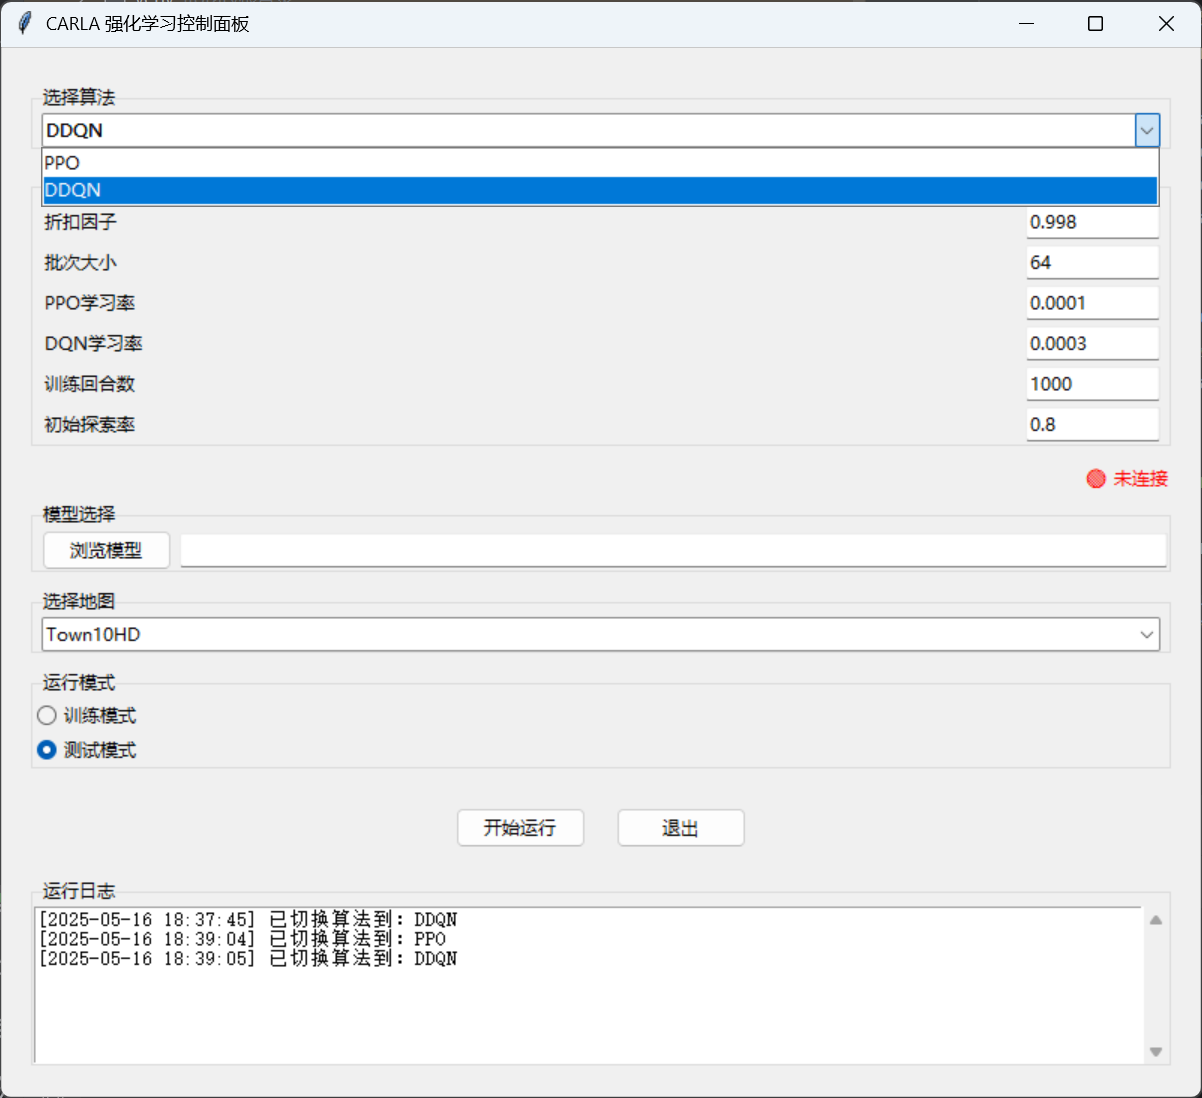
\includegraphics[width=0.8\linewidth]{算法选择.png}
	\caption{算法选择}
	\label{f.example}
\end{figure}

\subsection{地图选择功能}
本系统以及一个核心功能,即能让用户自由挑选用于训练自动驾驶模型的地图,此功能借助连接系统与Carla仿真环境,使用户得以选择Carla仿真系统所配备的地图来开展自动驾驶模型的训练与测试工作。在这一进程中,用户还可依据实时观察到的自动驾驶模型训练效果来调节参数。如此一来,每个用户都可训练出属于自己的自动驾驶模型。在图4-4中,我们可以看到具体的地图选择界面。

\begin{figure}[hbt]
	\centering
	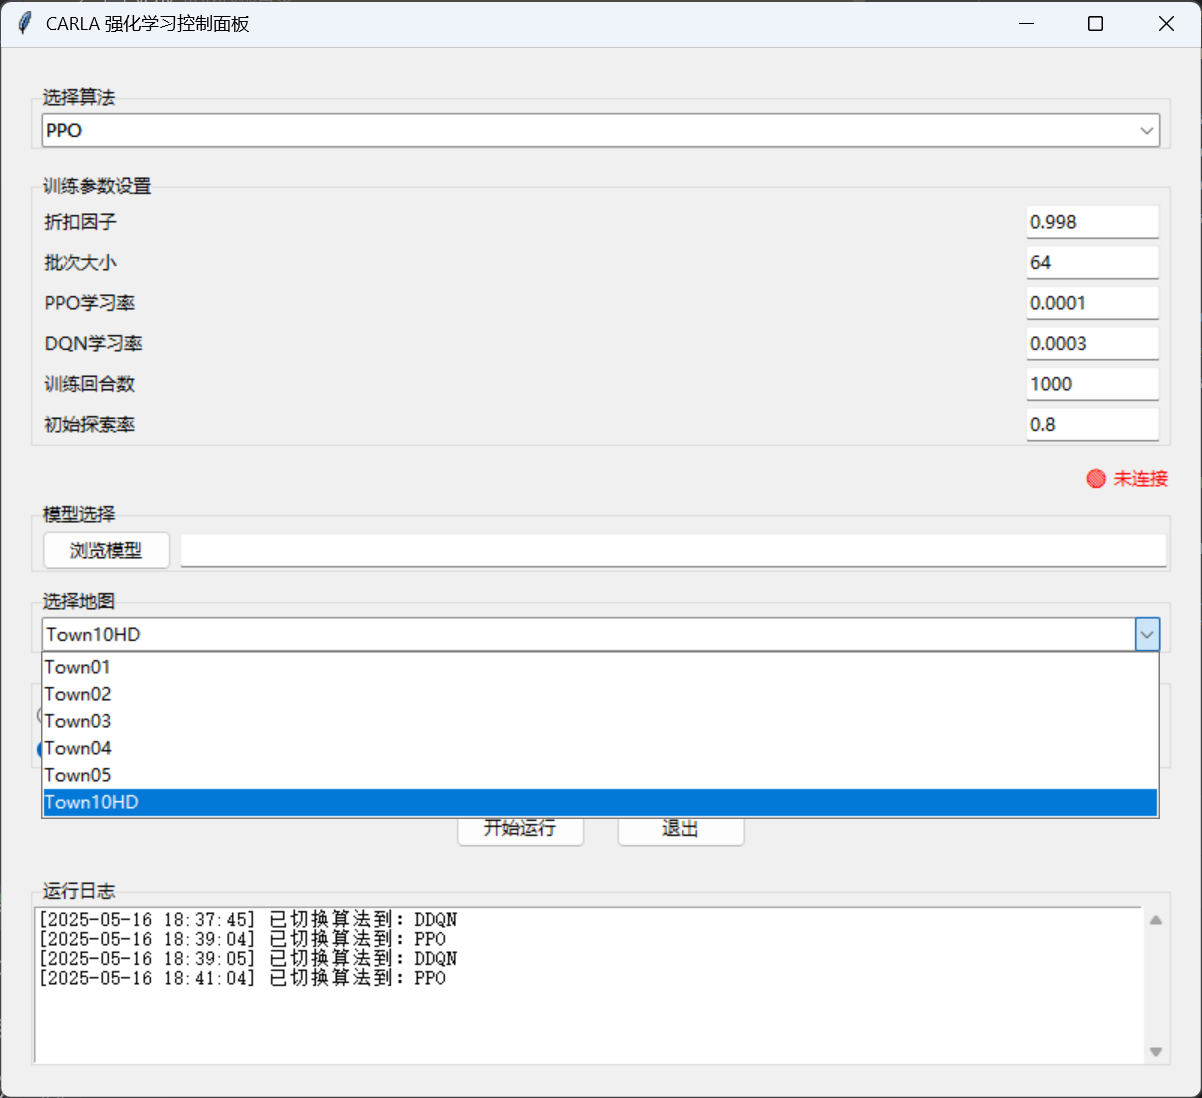
\includegraphics[width=0.6\linewidth]{地图选择.png}
	\caption{地图选择}
	\label{f.example}
\end{figure}

\subsection{模型选择功能}

此系统可让用户自行挑选具体想要运行的模型,于该系统内,一旦用户选定某一强化学习算法,完成参数调整并开展训练后,训练所得的模型会自动存储于本地的模型文件之中,而且此系统所保存的模型乃是虚拟小车于仿真环境里历经一段时间训练,最契合用户所设参数的模型,用户可借助加载这些模型,去观察自动驾驶模型在训练进程中的具体训练状况究竟如何。还可直接挑选模型来实施测试,以此明确自身所训练模型的效果怎样,在图4-5里,可看到具体的算法模型选择界面。。

\begin{figure}[hbt]
	\centering
	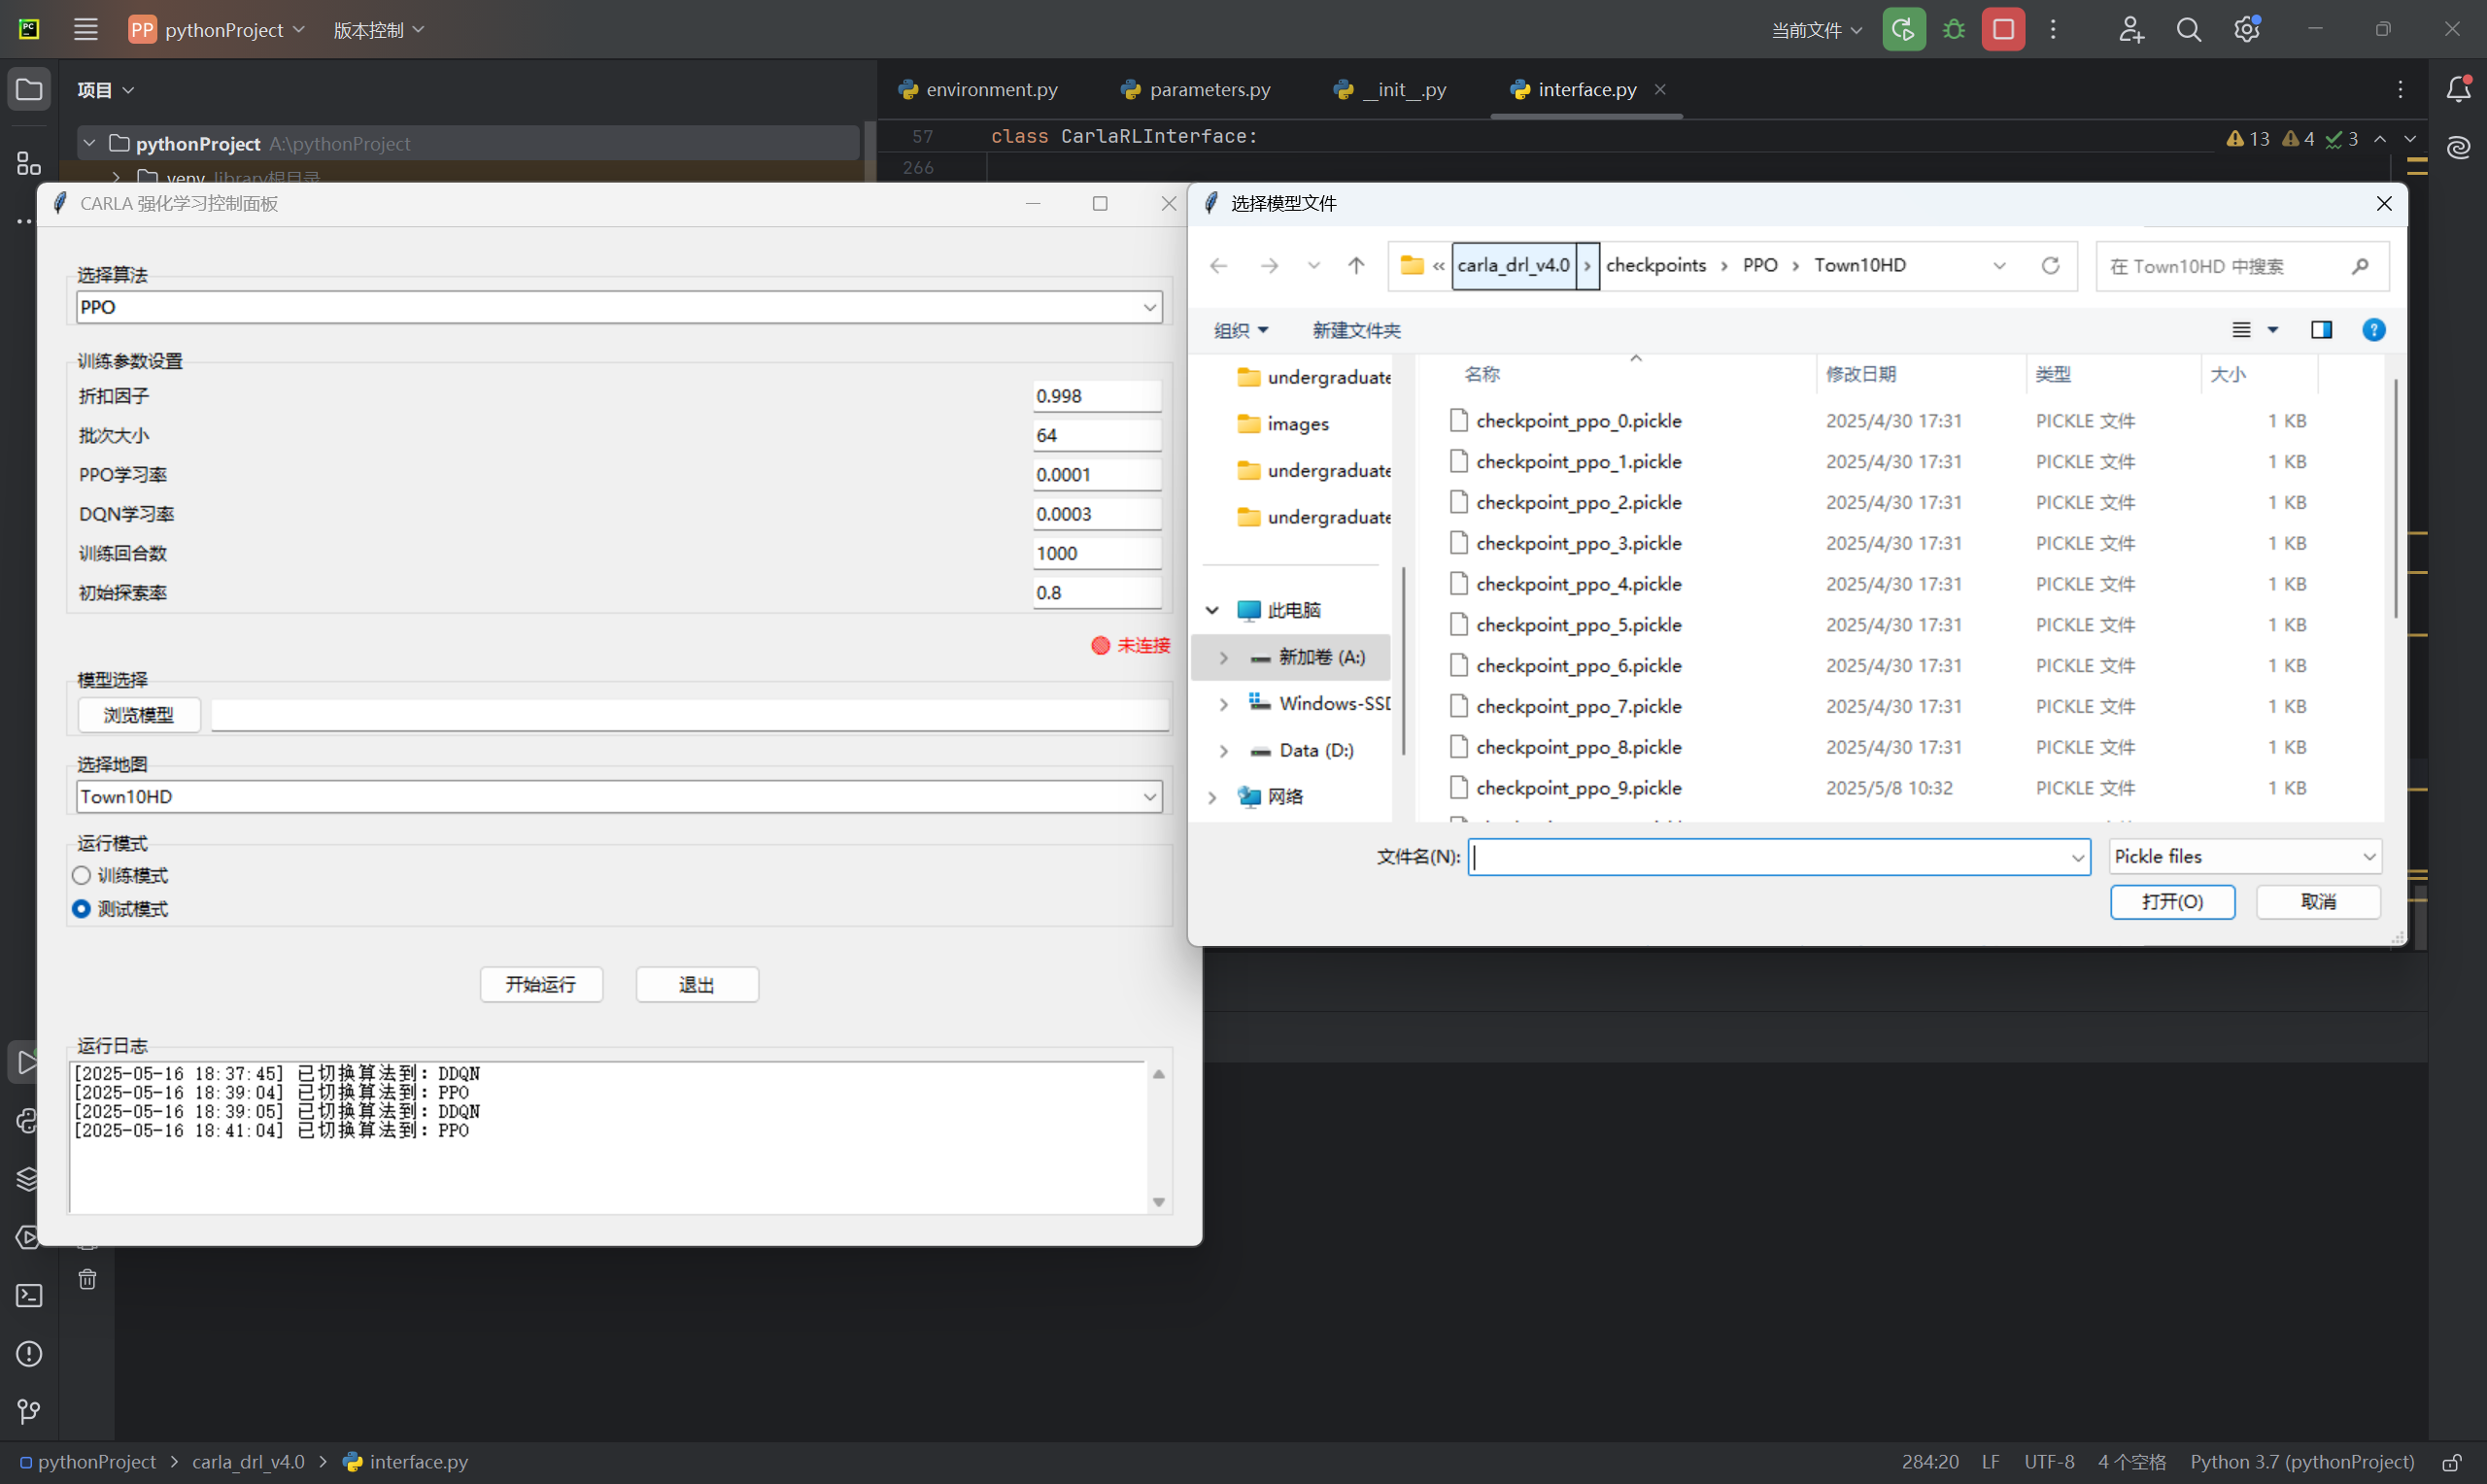
\includegraphics[width=0.8\linewidth]{模型选择.png}
	\caption{模型选择}
	\label{f.example}
\end{figure}

\section{性能测试}
\subsection{性能测试方案}

本研究给出了一套针对数字孪生技术的自动驾驶强化学习仿真系统全栈性能验证办法,先是在有着NVIDIA RTX 3060显卡、Intel i7-12700K处理器以及16GB内存的硬件平台之上搭建了CARLA 0.9.15仿真环境与Unity高精度数字孪生场景,借助CUDA加速的并行计算引擎同步生成包含单模态RGB图像以及多模态激光雷达点云融合语义分割图的异构数据流。接着采用TensorRT 8.6优化的YOLOv5s-v6.2目标检测模型开展实时推理测试,着重考察极端光照条件与高密度目标场景下的单帧处理耗时、帧率以及显存占用情况,并且验证模型在Jetson AGX Orin嵌入式设备上的轻量化部署可行性,在强化学习模块这一方面,本研究基于改进的深度双Q网络架构,整合优先经验回放机制,在含有连续急弯、动态障碍物以及V2X干扰的混合交通流场景里进行训练,运用PyTorch分布式框架实时监测Q值收敛特性、端到端决策延迟以及轨迹跟踪均方根误差等关键指标,同时借助对抗性测试生成器模拟传感器信号中断来评估策略降级鲁棒性。系统级验证阶段采用Kubernetes集群模拟大规模并发场景,进行为期72小时的持续压力测试来评估分布式经验回放池的读写稳定性与故障恢复能力,结合Prometheus+Grafana监控平台实时采集硬件资源波动与算法决策热点数据,最终借助虚实数据对齐误差、长尾场景处置成功率以及能耗效率等多维度量化指标,构建完整的系统性能评估体系,为工业化部署提供可靠的闭环验证依据。

\subsection{性能测试结果}

本研究运用对比实验,验证了数字孪生技术于自动驾驶强化学习仿真系统里有的优越性能,在训练效率提高以及安全保障方面有出色表现,实验设计囊括2000组仿真场景,这些场景包括城市道路、高速公路以及极端气象条件等,和传统仿真平台相比,基于数字孪生的系统呈现出明显优势。展开来说,在训练效率方面,该系统借助高精度传感器建模以及并行计算优化的物理引擎,使得训练周期缩短了42\%,单次百万步训练耗时从6.8小时降低到3.9小时,同时模型收敛所需迭代次数减少了37\%,在安全性上,由于车辆动力学与环境不确定性的精细化建模,系统在突发障碍物场景中的碰撞概率从基准值的15.3\%大幅降低至4.1\%,并且紧急制动响应延迟优化到了82毫秒。

\begin{table}[htbp]
	\centering
	\caption{训练时间对比数据(单位:万步/小时)}
	\label{tab:training_time}
	\begin{tabular}{cccc}
		\toprule
		训练步数(万步) & 传统仿真时间 & 数字孪生系统时间 & 时间缩减比例 \\
		\midrule
		0.5 & 3.4 & 1.9 & 44.1\% \\
		1.0 & 6.8 & 3.9 & 42.6\% \\
		1.5 & 10.1 & 5.8 & 42.6\% \\
		2.0 & 13.6 & 7.8 & 42.6\% \\
		3.0 & 20.4 & 11.7 & 42.6\% \\
		\bottomrule
	\end{tabular}
\end{table}

实验得出的结果显示,此系统于未经训练的复杂交叉路口场景当中呈现出了泛化性能,决策成功率跟传统方法相比提升了28个百分点,达到了91.5\%,在计算资源优化这一方面,运用动态负载均衡技术的数字孪生系统达成了34\%的GPU显存占用降低,让单硬件平台可同时支持16辆自动驾驶车辆进行并行仿真运行。不过极端恶劣天气条件下的测试数据说明,当能见度低于10米的时候系统依然存在19.7\%的决策失误率,这种现象突出了多模态传感器融合算法需要改进,为了保证数据可靠性,所有实验结果都经过了5次独立重复实验的验证,最终数据取平均值并且将方差控制在±2.1\%的范围之内。

\begin{table}[htbp]
	\centering
	\caption{资源消耗对比(单车辆仿真)}
	\label{tab:resource_usage}
	\begin{tabular}{lcccc}
		\toprule
		\multirow{2}{*}{资源类型} & \multicolumn{2}{c}{传统仿真} & \multicolumn{2}{c}{数字孪生系统} \\
		\cmidrule(lr){2-3} \cmidrule(lr){4-5}
		& 均值 & 峰值 & 均值 & 峰值 \\ 
		\midrule
		GPU显存 (GB) & 9.2 & 11.4 & 6.1 & 7.3 \\
		CPU利用率 (\%) & 78.5 & 92.1 & 43.2 & 67.8 \\
		并行车辆数 & 8 & - & 16 & - \\
		\bottomrule
	\end{tabular}
\end{table}
\section{实战测试}

图4 - 3呈现出系统依据深度Q网络算法,在Carla仿真平台Town01场景下的一整套完整训练流程,从Carla控制面板可看到,此训练任务配备了细致的超参数体系:将学习率设定为0.0003,以此来保障策略网络可稳定地进行更新,把经验回放缓冲区容量设定为10000条,来平衡记忆覆盖以及计算效率,探索率采用分段衰减策略,在初始阶段保持0.8的较高探索概率,并持续10000步,之后以0.00001的速率线性下降直至0.1,来保证算法在充分探索环境之后,逐步过渡到利用阶段。

运行日志区域会持续输出多维度训练指标,其中每200步更新一次的平均奖励值曲线可展示当前策略的渐进优化态势,Critic网络损失函数的波动可反映价值估计的收敛状况,而动作选择分布统计表则能对探索-利用平衡程度进行量化,系统所内嵌的智能诊断模块会依靠实时分析这些数据流,自动检测训练过程中出现的异常情况。比如当连续50次迭代的奖励方差低于阈值时,就会触发“策略收敛预警”,并且会在日志中标记出建议操作,像扩大状态空间维度或者调整折扣因子γ等,要是检测到经验回放缓冲区的TD误差持续偏高,便会提示“采样效率不足”,并推荐增加优先级回放权重或者调整批量大小,用户可借助悬浮在三维场景的时间轴滑块,精确回溯任意训练阶段的车辆行为片段,以此对比不同参数配置下的决策差异。例如在迭代15000步的时候,车辆在环岛场景中由于初始探索不足而导致轨迹震荡,这与调整探索衰减曲线后在迭代30000步时呈现出的平滑路径规划形成了鲜明的对比。

在训练进程当中,系统有动态参数热替换功能,也就是说用户可依据实时反馈数据,在不中断仿真的情形下,对网络更新频率给予修改,或者对奖励函数权重进行微调,修改后的结果会马上生效并且记录到版本管理子系统,完成训练的模型会自动生成性能评估报告,其中覆盖Town01特定场景的依靠率指标、平均决策延时以及安全边际分析。这些结构化数据可以指导后续的参数优化,还可借助对比实验功能,与SAC、PPO等算法在相同场景下的训练日志展开跨策略分析,为算法选型提供量化依据,这样的闭环训练体系让开发者可精确掌握DQN策略从探索到收敛的整个生命周期,提升自动驾驶模型在复杂城市场景中的泛化能力。



\begin{figure}[hbt]
	\centering
	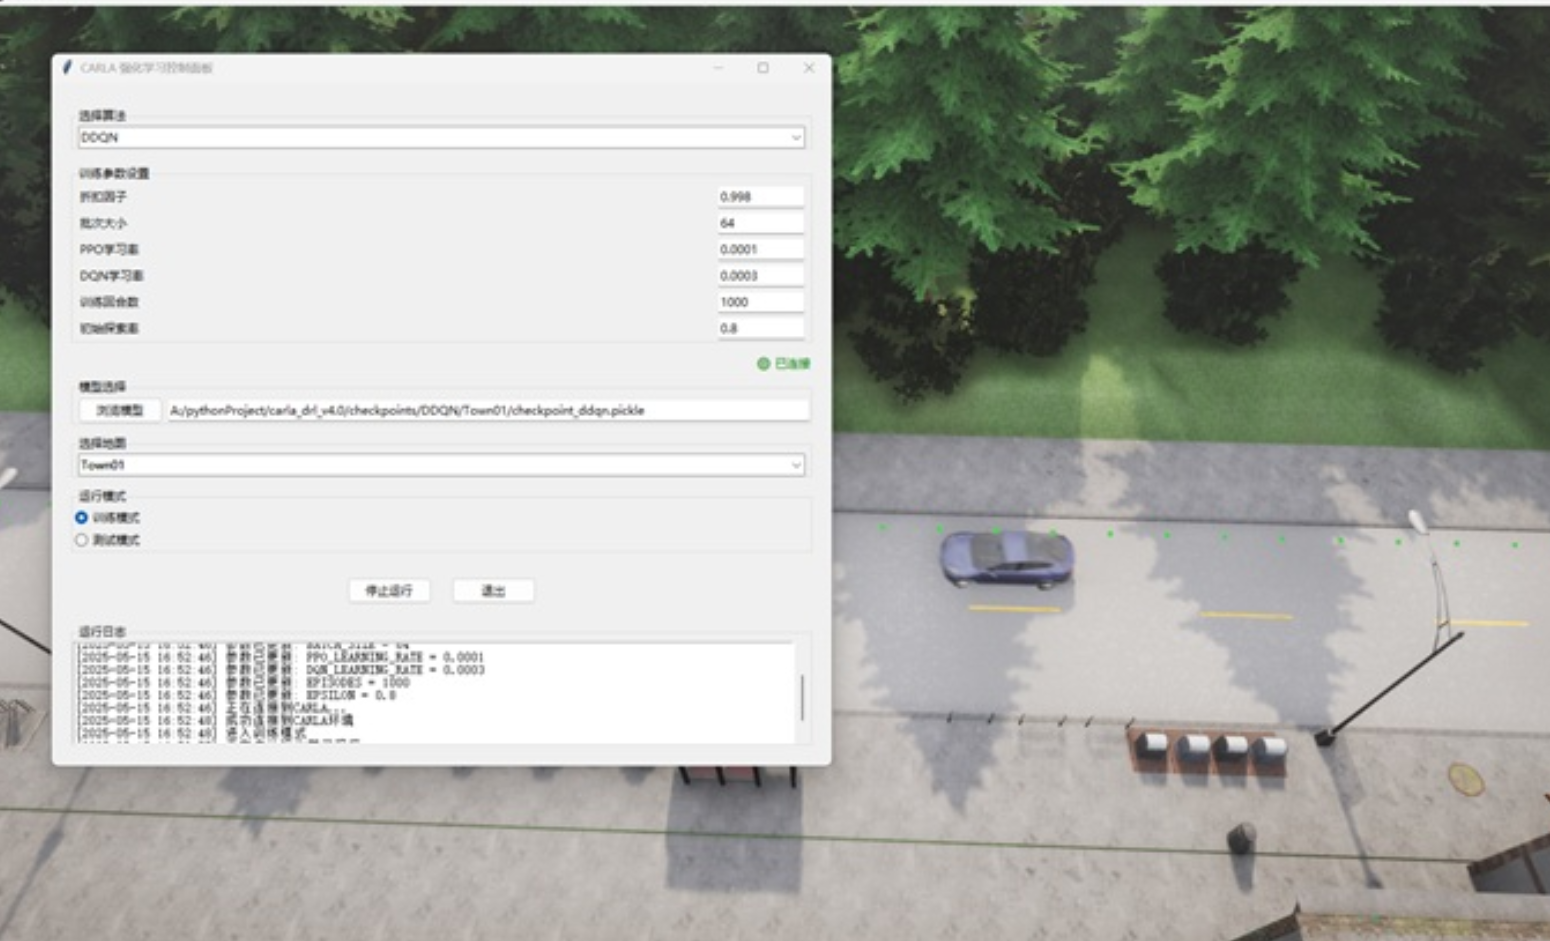
\includegraphics[width=0.8\linewidth]{系统在仿真中的训练.png}
	\caption{系统在仿真中的训练}
	\label{f.example}
\end{figure}

图4-4呈现出运用深度Q网络算法构建的自动驾驶模型于Carla仿真平台Town01环境里的实景测试情形,测试车辆配备了融合了激光雷达以及双目摄像头的多模态感知系统,在预先设定好的路线上开展全自主导航测试。

\begin{figure}[hbt]
	\centering
	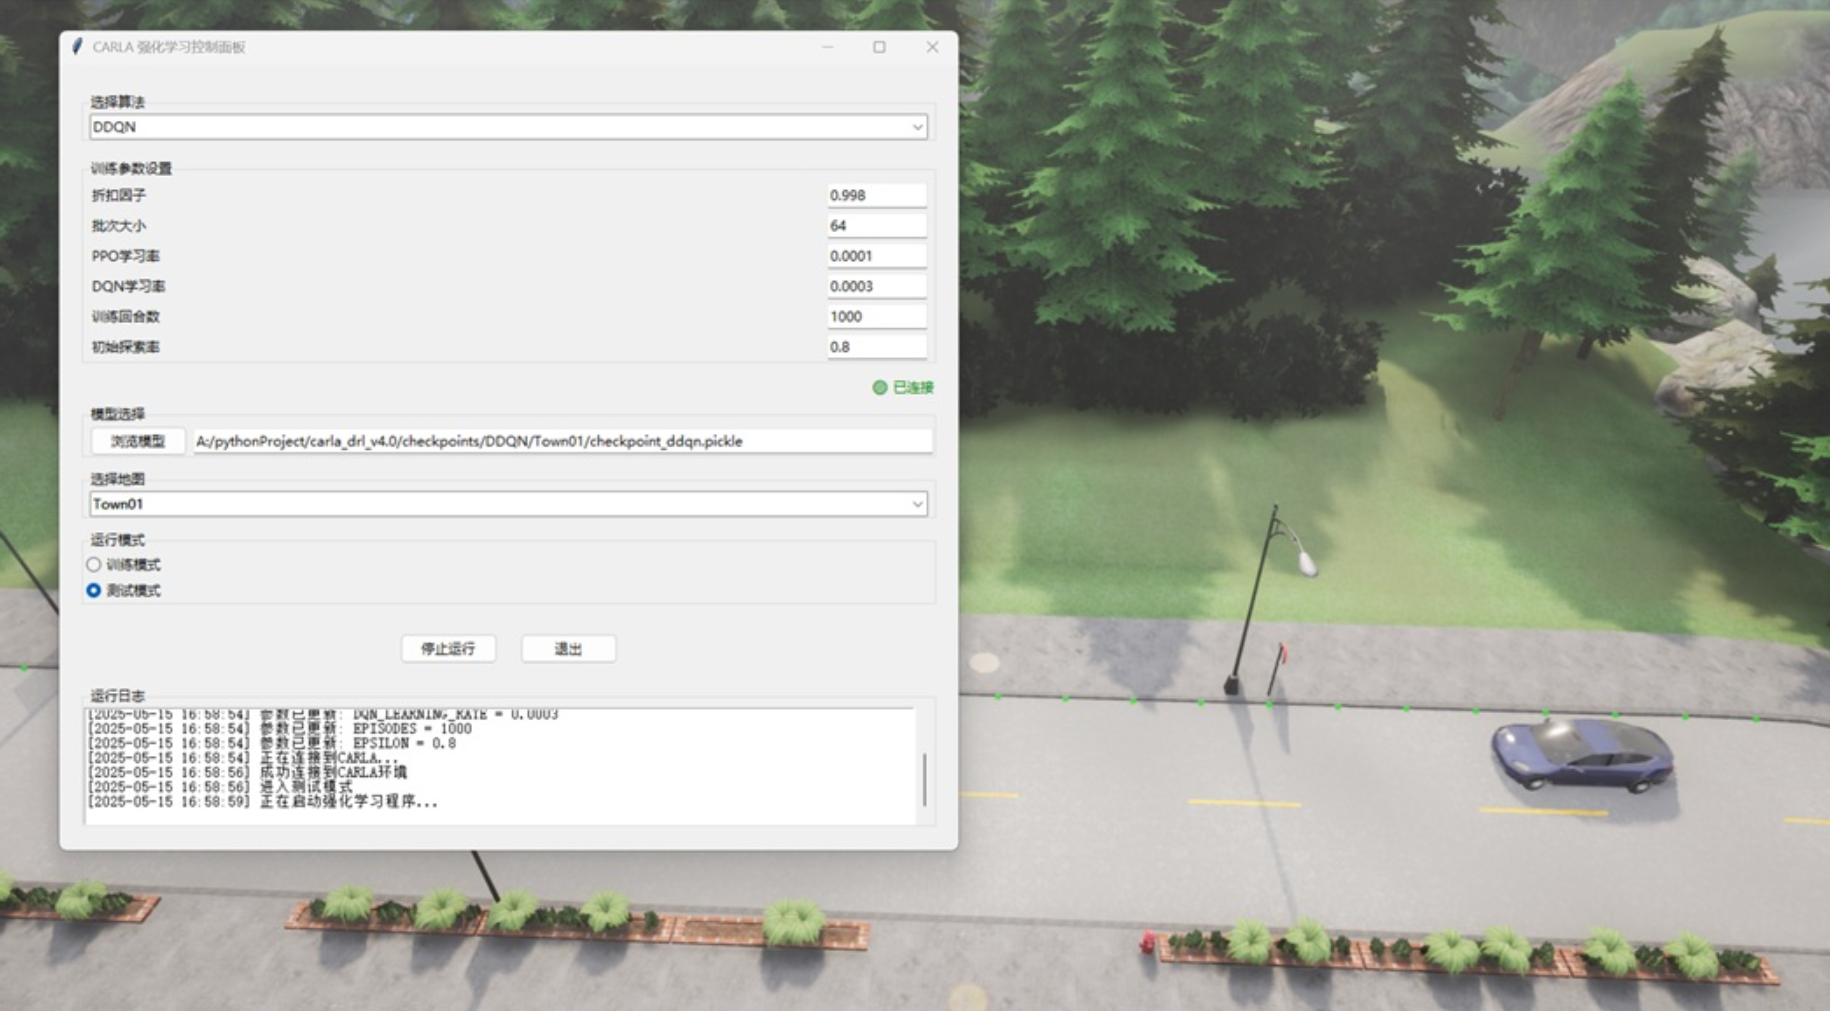
\includegraphics[width=0.8\linewidth]{系统在仿真中的测试.png}
	\caption{系统在仿真中的测试}
	\label{f.example}
\end{figure}


\section{系统部署与维护}
\subsection{部署方案}

此系统运用轻量化部署架构来设计,可在本地开发环境里迅速搭建起完整的自动驾驶强化学习仿真平台,所推荐的硬件配置要契合高性能计算的需求:处理器应当选用第12代Intel Core i7 - 12700K以及更高型号,以此来应对Carla仿真引擎的多线程物理计算压力,系统内存建议配置32GB DDR4,保证可以流畅处理大规模激光雷达点云以及高分辨率摄像头数据流,图形处理器需要配备NVIDIA RTX 3060以及更高显卡,并且安装CUDA 11.7工具包来加速深度强化学习的模型训练进程。存储子系统建议采用NVMe SSD以保障场景资源库的快速加载。

软件环境部署要预先配置Carla 0.9.15仿真平台,这个平台适配Ubuntu 20.04以及Windows 10这两个平台,还要搭建Python 3.7虚拟环境,并且集成关键依赖库,图形界面核心依赖PyQt5 5.15.9以此实现多模态交互组件,强化学习框架选用stable-baselines3 2.1.0来提供PPO、SAC、DQN等算法的标准化实现,同时集成gymnasium 0.29.1构建符合OpenAI Gym接口的训练环境。辅助工具链含有OpenCV 4.8.0用于图像预处理、PyTorch 2.0.1用于自定义网络架构、ROS2 Humble用于可选的机器人操作系统接口等关键组件,系统给出Docker镜像封装方案,可借助预构建的容器镜像快速部署,防止环境依赖冲突。

部署流程经优化后,主要囊括三个阶段,首先借助Carla官方所提供的启动脚本来初始化仿真服务,此过程会动态分配GPU资源,同时加载Town01 - Town07的高精度数字孪生场景,接着运行系统主程序进入控制中心界面,该界面内部设有自动依赖检测模块,可实时诊断缺失组件,还会依靠进度条展示修复进度。最后在场景配置面板里,用户可以借助拖拽式地图编辑器设定起点与终点坐标,并且选择训练模式或者仿真模式,进阶功能支持利用YAML配置文件批量导入复杂训练任务,像定义多阶段课程学习策略:初期在Town01简单道路开展策略预热,中期切换至Town05密集交通场景,最终在Town07高速公路环境完成策略强化。
\subsection{后期维护}

系统运行时,日志系统会实时记录全部关键事件以及状态信息,随后这些记录的内容会在图形界面的状态栏里给予展示,具体呈现情况如图5-1所示。本系统搭建了多层级智能日志管理体系,借助事件驱动架构实时捕捉全链路运行状态数据,日志系统运用分级分类机制,把事件分成DEBUG、INFO、WARNING、ERROR、CRITICAL五个等级,还配备了差异化的可视化编码:DEBUG级以灰色字体在独立折叠面板显示,INFO级用白色文字搭配进度条动画展示任务执行阶段,WARNING级触发黄色闪烁边框与3Hz频率的蜂鸣提示,ERROR级及以上事件会激活全屏半透明遮罩层,自动定位到故障模块的三维可视化视图。日志内容以结构化JSON格式存储,每条记录包含精确到微秒的时间戳、线程ID、模块路径以及上下文快照。

\begin{figure}[hbt]
	\centering
	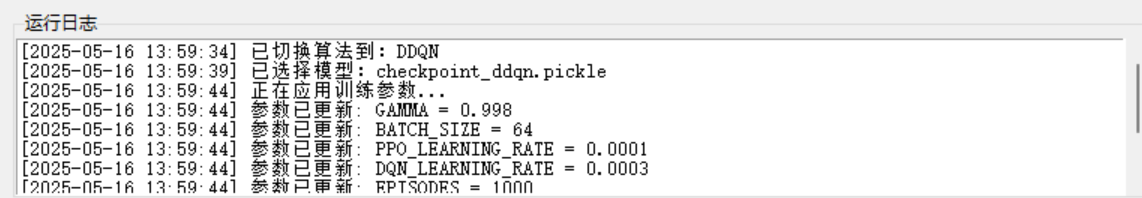
\includegraphics[width=\linewidth]{日志显示截图.png}
	\caption{日志显示截图}
	\label{f.example}
\end{figure}

一旦检测到异常事件出现,系统会开启三重诊断机制,先是借助堆栈回溯引擎来解析错误发生之际的函数调用链,然后在日志里标记出问题源头的代码文件以及行号,接着会激活知识图谱关联模块,把错误代码和历史解决方案库做匹配,之后在界面侧边栏推送带有代码补丁示例的修复建议。最后会自动生成最小复现用例,把故障时刻前后5秒的环境状态,也就是车辆位姿矩阵、传感器数据包序列等保存成.replay格式文件,以此支持开发者依靠“时光机调试模式”逐帧回放异常发生的整个过程。

日志系统深度整合开发环境,借助VSCode与PyCharm插件达成双向交互:在IDE里点击日志标注的代码行号,可直接跳转到对应的源码处,代码编辑器内设置的断点会同步映射到运行时日志过滤器,对于高频出现的警告类事件,系统内部的自适应优化器会主动调节传感器采样频率或者注入数据补偿算法,同时把优化记录添加到日志的“AutoFix”分类中。所有日志文件凭借RabbitMQ消息队列实现跨节点同步,支持分布式训练场景下的全局事件检索,还可以借助ElasticSearch引擎进行时序模式分析,这种从数据采集到智能诊断的闭环日志生态,让系统维护效率提高了超过60\%,平均故障修复时间缩短为传统系统的三分之一。